\documentclass{article}
\usepackage[utf8]{inputenc}
\usepackage[a4paper, margin=0.75in]{geometry}
\usepackage{CJKutf8}
\usepackage{amsmath,amssymb}
\usepackage{setspace}
\usepackage{graphicx}
\graphicspath{{./images/}}

\setstretch{3}

\begin{document}

\begin{CJK*}{UTF8}{bkai}
    \begin{center}
        {\Huge \textbf{Computer Organization Lab06 Report}} \\
        {\large \textbf{Author:} 109652039 林立倫, 109550003 陳茂祥}
    \end{center}
\end{CJK*}

\section{Implementation}
\subsection{Direct Mapped}
First, we need to analyze how the address is constructed. We calculate the length of tag, index, and block offset in the address by \verb|get_indexing_size|. 
Second, we construct our cache by a vector of \verb|Block|, which consists of a valid bit and a tag.
Then, read the address from file and seperate them into tag, index and block offset by function \verb|get_bits|.
If the block is not valid or the tag is not the same as the current one, there is a read miss. Otherwise, it is a read hit.
Finally, we calculate the hit rate and return the result.

\subsection{Set Associative}
First, we also analyze the composition of address. But this time, we construct our cache by vector of \verb|Set|.
\verb|Set| contains a vector of \verb|Block| to store valid bit and tags, a \verb|use| vector to store when the block is used last time, and a variable \verb|counter| to represent time.
Second, read address from the file and seperate them into tag, index and block offset by function \verb|get_bits|.
Then, we call the function \verb|add_block| for further process. In this function, if the tag is found in the corresponding set, we will update the time in \verb|use| and return true. 
Otherwise, if the set is not full, we simply add it to the set, update the \verb|use| value and return false. 
For those situations with full set, we replace the block by \verb|LRU| and return false. 
Finally, we can calculate the hit time and the hit rate by the return value of the \verb|add_block| function.

\newpage
\section{Result}
\begin{figure}[!htb]
    \centering
    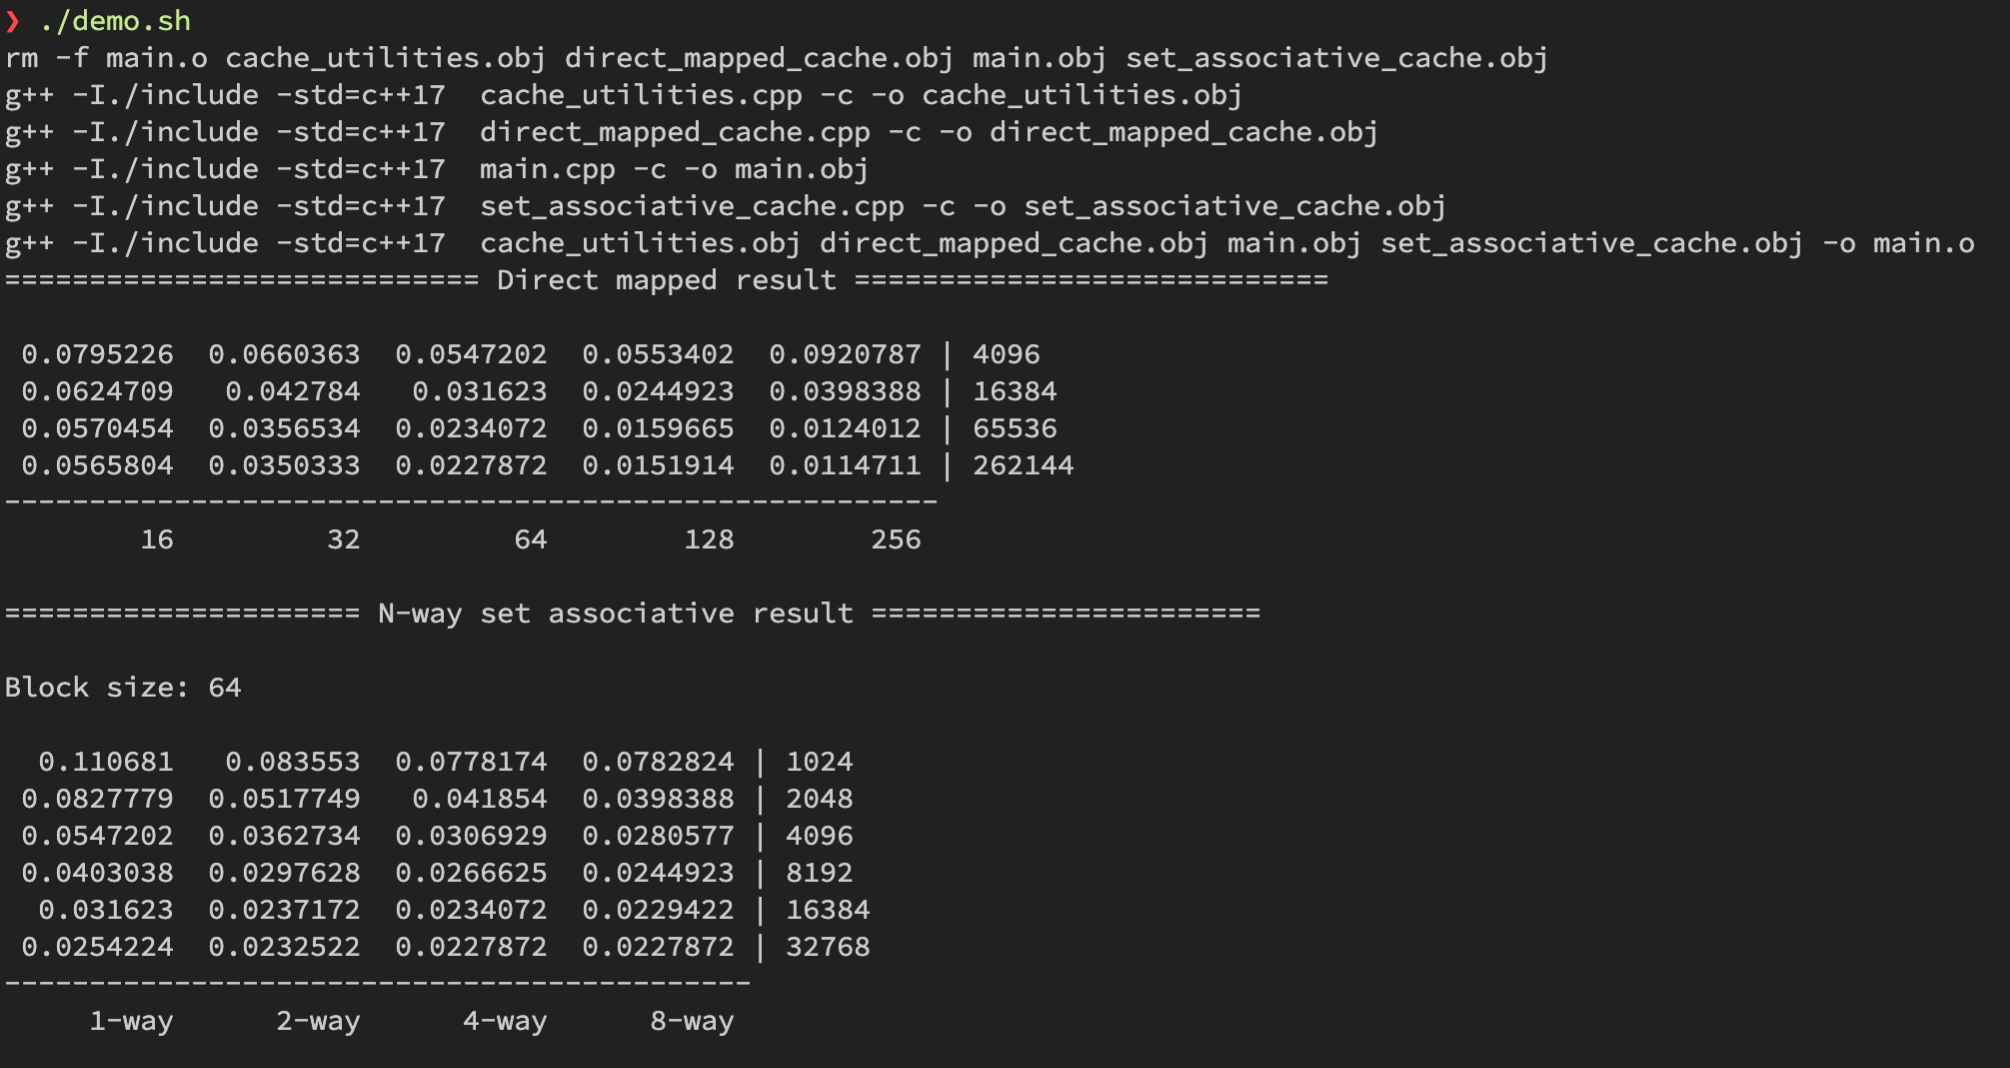
\includegraphics[width=0.75\textwidth]{result.png}
\end{figure}
\section{Problems and Solution}
Because we want to seperate the functions from the original cpp files, we add a header file for function declaration and another cpp file for function definition.
Thus, we need to modify Makefile to compile with these additional files. Thanks to TAs for answering questions soonly. At the end of this class, thanks to Prof. T.F.Chen for the great class and TAs for helpful assistance.
\end{document}